% This file was converted to LaTeX by Writer2LaTeX ver. 1.0.2
% see http://writer2latex.sourceforge.net for more info
\documentclass[letterpaper]{article}
\usepackage[latin1]{inputenc}
\usepackage[T1]{fontenc}
\usepackage[english]{babel}
\usepackage{amsmath}
\usepackage{amssymb,amsfonts,textcomp}
\usepackage{color}
\usepackage{array}
\usepackage{supertabular}
\usepackage{hhline}
\usepackage{hyperref}
\hypersetup{pdftex, colorlinks=true, linkcolor=blue, citecolor=blue, filecolor=blue, urlcolor=blue, pdftitle=SYSTEMS AND SOFTWARE REQUIREMENTS SPECIFICATION (SSRS) TEMPLATE, pdfauthor=Clinton Jeffery, pdfsubject=, pdfkeywords=}
\usepackage[pdftex]{graphicx}
% Text styles
\newcommand\textstyleDefaultParagraphFont[1]{#1}
\newcommand\textstyleHyperlink[1]{\textcolor{blue}{#1}}
\newcommand\textstylePageNumber[1]{#1}
% Outline numbering
\setcounter{secnumdepth}{5}
\renewcommand\thesection{\arabic{section}}
\renewcommand\thesubsection{\arabic{section}.\arabic{subsection}}
\renewcommand\thesubsubsection{\arabic{section}.\arabic{subsection}.\arabic{subsubsection}}
\renewcommand\theparagraph{\arabic{section}.\arabic{subsection}.\arabic{subsubsection}.\arabic{paragraph}}
\renewcommand\thesubparagraph{\arabic{section}.\arabic{subsection}.\arabic{subsubsection}.\arabic{paragraph}.\arabic{subparagraph}}
\makeatletter
\newcommand\arraybslash{\let\\\@arraycr}
\makeatother
% List styles
\newcounter{saveenum}
\newcommand\liststyleLi{%
\renewcommand\theenumi{\arabic{enumi}}
\renewcommand\theenumii{\alph{enumii}}
\renewcommand\theenumiii{\roman{enumiii}}
\renewcommand\theenumiv{\arabic{enumiv}}
\renewcommand\labelenumi{\theenumi.}
\renewcommand\labelenumii{\theenumii.}
\renewcommand\labelenumiii{\theenumiii.}
\renewcommand\labelenumiv{\theenumiv.}
}
\newcommand\liststyleLii{%
\renewcommand\theenumi{\arabic{enumi}}
\renewcommand\theenumii{\alph{enumii}}
\renewcommand\theenumiii{\roman{enumiii}}
\renewcommand\theenumiv{\arabic{enumiv}}
\renewcommand\labelenumi{\theenumi.}
\renewcommand\labelenumii{\theenumii.}
\renewcommand\labelenumiii{\theenumiii.}
\renewcommand\labelenumiv{\theenumiv.}
}
\newcommand\liststyleLiii{%
\renewcommand\theenumi{\arabic{enumi}}
\renewcommand\theenumii{\alph{enumii}}
\renewcommand\theenumiii{\roman{enumiii}}
\renewcommand\theenumiv{\arabic{enumiv}}
\renewcommand\labelenumi{\theenumi.}
\renewcommand\labelenumii{\theenumii.}
\renewcommand\labelenumiii{\theenumiii.}
\renewcommand\labelenumiv{\theenumiv.}
}
\newcommand\liststyleLiv{%
\renewcommand\theenumi{\arabic{enumi}}
\renewcommand\theenumii{\alph{enumii}}
\renewcommand\theenumiii{\roman{enumiii}}
\renewcommand\theenumiv{\arabic{enumiv}}
\renewcommand\labelenumi{\theenumi.}
\renewcommand\labelenumii{\theenumii.}
\renewcommand\labelenumiii{\theenumiii.}
\renewcommand\labelenumiv{\theenumiv.}
}
\newcommand\liststyleLv{%
\renewcommand\theenumi{\arabic{enumi}}
\renewcommand\theenumii{\alph{enumii}}
\renewcommand\theenumiii{\roman{enumiii}}
\renewcommand\theenumiv{\arabic{enumiv}}
\renewcommand\labelenumi{\theenumi.}
\renewcommand\labelenumii{\theenumii.}
\renewcommand\labelenumiii{\theenumiii.}
\renewcommand\labelenumiv{\theenumiv.}
}
\newcommand\liststyleLvi{%
\renewcommand\theenumi{\arabic{enumi}}
\renewcommand\theenumii{\alph{enumii}}
\renewcommand\theenumiii{\roman{enumiii}}
\renewcommand\theenumiv{\arabic{enumiv}}
\renewcommand\labelenumi{\theenumi.}
\renewcommand\labelenumii{\theenumii.}
\renewcommand\labelenumiii{\theenumiii.}
\renewcommand\labelenumiv{\theenumiv.}
}
\newcommand\liststyleLvii{%
\renewcommand\theenumi{\alph{enumi}}
\renewcommand\theenumii{\alph{enumii}}
\renewcommand\theenumiii{\roman{enumiii}}
\renewcommand\theenumiv{\arabic{enumiv}}
\renewcommand\labelenumi{\theenumi.}
\renewcommand\labelenumii{\theenumii.}
\renewcommand\labelenumiii{\theenumiii.}
\renewcommand\labelenumiv{\theenumiv.}
}
\newcommand\liststyleLviii{%
\renewcommand\theenumi{\arabic{enumi}}
\renewcommand\theenumii{\alph{enumii}}
\renewcommand\theenumiii{\roman{enumiii}}
\renewcommand\theenumiv{\arabic{enumiv}}
\renewcommand\labelenumi{\theenumi.}
\renewcommand\labelenumii{\theenumii.}
\renewcommand\labelenumiii{\theenumiii.}
\renewcommand\labelenumiv{\theenumiv.}
}
\newcommand\liststyleLix{%
\renewcommand\theenumi{\arabic{enumi}}
\renewcommand\theenumii{\alph{enumii}}
\renewcommand\theenumiii{\roman{enumiii}}
\renewcommand\theenumiv{\arabic{enumiv}}
\renewcommand\labelenumi{\theenumi.}
\renewcommand\labelenumii{\theenumii.}
\renewcommand\labelenumiii{\theenumiii.}
\renewcommand\labelenumiv{\theenumiv.}
}
\newcommand\liststyleLFOxiii{%
\renewcommand\theenumi{}
\renewcommand\labelenumi{\theenumi}
\renewcommand\labelitemi{[F0B7?]}
\renewcommand\labelitemii{o}
\renewcommand\labelitemiii{[F0A7?]}
}
\newcommand\liststyleLx{%
\renewcommand\theenumi{\arabic{enumi}}
\renewcommand\theenumii{\alph{enumii}}
\renewcommand\theenumiii{\roman{enumiii}}
\renewcommand\theenumiv{\arabic{enumiv}}
\renewcommand\labelenumi{\theenumi.}
\renewcommand\labelenumii{\theenumii.}
\renewcommand\labelenumiii{\theenumiii.}
\renewcommand\labelenumiv{\theenumiv.}
}
% Page layout (geometry)
\setlength\voffset{-1in}
\setlength\hoffset{-1in}
\setlength\topmargin{0.7874in}
\setlength\oddsidemargin{0.7874in}
\setlength\textheight{8.625199in}
\setlength\textwidth{6.9251995in}
\setlength\footskip{0.3in}
\setlength\headheight{0.5in}
\setlength\headsep{0cm}
% Footnote rule
\setlength{\skip\footins}{0.0469in}
\renewcommand\footnoterule{\vspace*{-0.0071in}\setlength\leftskip{0pt}\setlength\rightskip{0pt plus 1fil}\noindent\textcolor{black}{\rule{0.25\columnwidth}{0.0071in}}\vspace*{0.0398in}}
% Pages styles
\makeatletter
\newcommand\ps@MP{
  \renewcommand\@oddhead{\rmfamily University of Idaho CS Department Instructional Use\hfill \hfill NOT FOR RELEASE}
  \renewcommand\@evenhead{\@oddhead}
  \renewcommand\@oddfoot{\textstylePageNumber{SSRS Page }\textstylePageNumber{\thepage{}}}
  \renewcommand\@evenfoot{\@oddfoot}
  \renewcommand\thepage{\arabic{page}}
}
\newcommand\ps@MPF{
  \renewcommand\@oddhead{}
  \renewcommand\@evenhead{\@oddhead}
  \renewcommand\@oddfoot{}
  \renewcommand\@evenfoot{\@oddfoot}
  \renewcommand\thepage{\arabic{page}}
}
\newcommand\ps@Standard{
  \renewcommand\@oddhead{}
  \renewcommand\@evenhead{}
  \renewcommand\@oddfoot{}
  \renewcommand\@evenfoot{}
  \renewcommand\thepage{\arabic{page}}
}
\newcommand\ps@MPii{
  \renewcommand\@oddhead{\rmfamily University of Idaho CS Department Instructional Use\hfill \hfill NOT FOR RELEASE}
  \renewcommand\@evenhead{\@oddhead}
  \renewcommand\@oddfoot{\textstylePageNumber{SSRS Page }\textstylePageNumber{\thepage{}}}
  \renewcommand\@evenfoot{\@oddfoot}
  \renewcommand\thepage{\arabic{page}}
}
\makeatother
\pagestyle{Standard}
\setlength\tabcolsep{1mm}
\renewcommand\arraystretch{1.3}
\title{SYSTEMS AND SOFTWARE REQUIREMENTS SPECIFICATION (SSRS) TEMPLATE}
\author{Clinton Jeffery}
\date{2010-09-21T21:43:51.01}
\begin{document}
\clearpage\clearpage\setcounter{page}{1}\pagestyle{MP}
\thispagestyle{MPF}
{\centering\bfseries\color{black}
SYSTEMS AND SOFTWARE REQUIREMENTS SPECIFICATION (SSRS) FOR
\par}


\bigskip

{\centering\bfseries\color{black}
Groups in a University Setting
\par}


\bigskip

{\centering 

\includegraphics[width=3.4882in,height=2.3374in]{Gusspec-img1.jpg}
\par}


\bigskip


\bigskip


\bigskip

{\centering\bfseries\color{black}
Version 0.004
\par}

{\centering\bfseries\color{black}
Sept 10
\par}


\bigskip


\bigskip

{\centering\bfseries\color{black}
Prepared for:
\par}

{\centering\bfseries\color{black}
Dr. Clinton Jeffery
\par}


\bigskip


\bigskip

{\centering\bfseries\color{black}
Prepared by:
\par}

{\centering\bfseries\color{black}
Chandler A, Sasha K, Mike S, John S, Leah W
\par}

{\centering\bfseries\color{black}
University of Idaho
\par}

{\centering\bfseries\color{black}
Moscow, ID \ 83844-1010
\par}

\clearpage{\centering\bfseries\color{black}
gus SSRS
\par}

{\centering\bfseries\color{black}
TABLE OF CONTENTS
\par}


\bigskip

{\bfseries\color{black}
Section\ \ Page}

\setcounter{tocdepth}{9}
\renewcommand\contentsname{Table of Contents}
\tableofcontents
\clearpage\clearpage\setcounter{page}{1}\pagestyle{MPii}
{\centering\bfseries\color{black}
\textstyleDefaultParagraphFont{1. Introduction}
\par}

\subsection[IDENTIFICATION]{\rmfamily IDENTIFICATION}
{\color{black}
The software system being considered for development is referred to as
Groups in a University Setting or gus. \ The specifications for the
system are being developed by the team itself. \ The ultimate customer,
or end-user, of the system will be universities or similar institutions
including but not limited to the University of Idaho. \ This is a new
project effort, so the version under development is version 1.0.}

\subsection[PURPOSE]{\rmfamily PURPOSE}
{\color{black}
The purpose of the system under development is to provide a tool for the
easy administration and control of university-style groups including
but not limited to clubs and sports teams. \ While the system will be
used by university personnel, this document is intended to be read and
understood by UICS software designers and coders.}

\subsection[SCOPE]{\rmfamily SCOPE}
{\color{black}
\textstyleDefaultParagraphFont{1. Simplifying tasks down to things only
leaders of groups will be required to do, such as:}}

{\color{black}
\textstyleDefaultParagraphFont{a. Sending notifications to group members
(email)}}

{\color{black}
\textstyleDefaultParagraphFont{b. Sending information (files) to group
members via email or download link}}

{\color{black}
\textstyleDefaultParagraphFont{c. Managing a group-wide calendar of
events}}

{\color{black}
\textstyleDefaultParagraphFont{d. Automatically generating:}}

{\color{black}
\textstyleDefaultParagraphFont{i. Contact information (contact sheets,
phone directories)}}

{\color{black}
\textstyleDefaultParagraphFont{ii. Website with updated contact, group,
event, and customized information}}

{\color{black}
\textstyleDefaultParagraphFont{iii. Organization charts}}

{\color{black}
\textstyleDefaultParagraphFont{iv. Graphical relationships between
groups}}

{\color{black}
\textstyleDefaultParagraphFont{v. Fees, dues, and expenses
notifications}}

{\color{black}
\textstyleDefaultParagraphFont{2. Consolidating information for members
and potential members of groups:}}

{\color{black}
\textstyleDefaultParagraphFont{a. Common location of group information}}

{\color{black}
\textstyleDefaultParagraphFont{b. Searching existing groups}}

{\color{black}
\textstyleDefaultParagraphFont{c. Tying together existing groups (even
suggesting similar groups)}}

{\color{black}
\textstyleDefaultParagraphFont{d. Personalized emails regarding
changes/updates}}

{\color{black}
\textstyleDefaultParagraphFont{e. Outstanding expenses or
reimbursements}}

{\color{black}
\textstyleDefaultParagraphFont{f. Reliable (i.e., automatically
updated):}}

{\color{black}
\textstyleDefaultParagraphFont{i. Group contact information}}

{\color{black}
\textstyleDefaultParagraphFont{ii. Group event information}}

\subsection[DEFINITIONS, ACRONYMS, AND ABBREVIATIONS]{\rmfamily
DEFINITIONS, ACRONYMS, AND ABBREVIATIONS}

\bigskip

\begin{flushleft}
\tablehead{}
\begin{supertabular}{|m{1.3587599in}|m{4.9941597in}|}
\hline
\centering \bfseries\color{black} Term or Acronym &
\centering\arraybslash \bfseries\color{black} Definition\\\hline
\color{black} Alpha test &
\color{black} Limited release(s) to selected, outside testers\\\hline
\color{black} Beta test &
\color{black} Limited release(s) to cooperating customers wanting early
access to developing systems\\\hline
\color{black} Final test &
\color{black} aka, Acceptance test, release of full functionality to
customer for approval\\\hline
\color{black} DFD &
\color{black} Data Flow Diagram\\\hline
\color{black} SDD &
\color{black} Software Design Document, aka SDS, Software Design
Specification\\\hline
\color{black} SRS &
\color{black} Software Requirements Specification\\\hline
\color{black} SSRS &
\color{black} System and Software Requirements Specification\\\hline
\color{black} gus &
\color{black} Groups in a University Setting\\\hline
\color{black} Member &
\color{black} A user who has an account and is considered to be part of
the group in question\\\hline
\color{black} Pseudo-member &
\color{black} A user who does not have an account of their own, but is
still considered to be part of the group in question\\\hline
\color{black} Group &
\color{black} A collection of groups and/or members that has an assigned
leader, or leaders\\\hline
\end{supertabular}
\end{flushleft}
\subsection[REFERENCES]{\rmfamily REFERENCES}
{\bfseries\color{black}
\textstyleDefaultParagraphFont{\textmd{gus proposal:}}
\href{http://www2.cs.uidaho.edu/~jeffery/courses/383/hw1/solomon_kopriva.pdf}{\textstyleHyperlink{\textmd{http://www2.cs.uidaho.edu/\~{}jeffery/courses/383/hw1/solomon\_kopriv}}}\href{http://www2.cs.uidaho.edu/~jeffery/courses/383/hw1/solomon_kopriva.pdf}{\textstyleHyperlink{\textmd{a}}}\href{http://www2.cs.uidaho.edu/~jeffery/courses/383/hw1/solomon_kopriva.pdf}{\textstyleHyperlink{\textmd{.pdf}}}\textstyleDefaultParagraphFont{\textmd{
}}}

\subsection[OVERVIEW AND RESTRICTIONS]{\rmfamily OVERVIEW AND
RESTRICTIONS}
{\color{black}
This document is for limited release only to UI CS personnel working on
the project.}


\bigskip

{\color{black}
Section 2 of this document describes the system under development from a
holistic point of view. \ Functions, characteristics, constraints,
assumptions, dependencies, and overall requirements are defined from
the system-level perspective.}


\bigskip

{\color{black}
Section 3 of this document describes the specific requirements of the
system being developed. \ Interfaces, features, and specific
requirements are enumerated and described to a degree sufficient for a
knowledgeable designer or coder to begin crafting an architectural
solution to the proposed system.}


\bigskip

{\color{black}
Section 4 provides the requirements traceability information for the
project. \ Each feature of the system is indexed by the SSRS
requirement number and linked to its SDD and test references.}


\bigskip

\section[Sections 5 and up are appendices including original information
and communications used to create this document.OVERALL
DESCRIPTION]{\textstyleDefaultParagraphFont{\textmd{Sections 5 and up
are appendices including original information and communications used
to create this document.}}\textstyleDefaultParagraphFont{OVERALL
DESCRIPTION}}
\subsection[PRODUCT PERSPECTIVE]{\rmfamily PRODUCT PERSPECTIVE}

\bigskip

{\color{black}
Gus is an independent software system, as it does not directly integrate
with a larger system. \ However, gus does draw data from external
sources, such as personal information databases, and needs to be
integrated with a web server in order to be readily accessible.}

\subsection[PRODUCT FUNCTIONS]{\rmfamily PRODUCT FUNCTIONS}

\bigskip

{\color{black}
Gus is a system for managing groups of people, specifically in a
university setting. \ It tries to maintain a balance between generality
and domain-specific paradigms. \ While gus could be used to manage
groups of people in any setting, it contains a set of defaults and
tunings specific to a university.}

{\color{black}
Managing people includes sending messages and files to groups of people,
automatically generating human and machine-readable information such as
contact sheets, organization charts, and calendars, helping people find
groups they would like to be a part of, automating fee and expense
notifications, and consolidating information about groups in an
automatically-generated web site.}


\bigskip

\subsection[USER CHARACTERISTICS]{\textstyleDefaultParagraphFont{USER
CHARACTERISTICS}}

\bigskip

{\color{black}
Gus should be easy for any user to understand with a brief explanation
and intuitive enough for an uninitiated user to figure out by looking
through the options. \ Basic computer use skills and a simple
conceptual explanation should be enough for every day usage.}

\subsection[CONSTRAINTS]{\rmfamily CONSTRAINTS}

\bigskip

{\color{black}
Gus needs to be able to interface with any data source it needs
information from, which could prove to be personnel databases and
authentication servers. \ It must support multiple user connections at
the same time. \ It should be reliable with little maintenance, and be
secure enough to be accessible by legitimate from the Internet proper.}

\subsection[ASSUMPTIONS AND DEPENDENCIES]{\rmfamily ASSUMPTIONS AND
DEPENDENCIES}
{\color{black}
It is assumed that the gus server will run on a Unix-like system, but it
may be necessary to port it to other operating systems. \ Enough
bandwidth to support the maximum estimated concurrent users must be
provided.}

\subsection[SYSTEM LEVEL (NON{}-FUNCTIONAL) REQUIREMENTS]{\rmfamily
SYSTEM LEVEL (NON-FUNCTIONAL) REQUIREMENTS}
\subsubsection[Site dependencies]{\rmfamily Site dependencies}
{\color{black}
Gus will need a Unix-like server to run on, with sufficient bandwidth
and processing power to serve the estimated number of concurrent users.
\ It will require a database in which to store its data.}

\subsubsection[Safety, security and privacy requirements]{\rmfamily
Safety, security and privacy requirements}
{\color{black}
Apart from standard security that servers connected to the Internet
require, gus will need a secure authentication system. \ Secure access
and authentication is important, but most of the security requirements
are related to access, and will be handled by the hierarchy of people
in charge. \ Gus cannot prevent a group leader from distributing
contact information, but it can provide a framework for disallowing
unauthorized access to the information.}

\subsubsection[Performance requirements]{\rmfamily Performance
requirements}
{\color{black}
Gus must be able to handle at least thirty-five simultaneous users with
all transactions visible to the user within one second (given ideal
network speeds).}

\subsubsection[System and software quality]{\rmfamily System and
software quality}
{\color{black}
Gus must perform all required functions, behave consistently and
correctly, be easily corrected, always running, generalized enough to
be easily adaptable, test-driven, and easy to use.}

\subsubsection[Packaging and delivery requirements]{\rmfamily Packaging
and delivery requirements}
{\color{black}
The executable system and all associated documentation (i.e., SSRS, SDD,
code listing, test plan (data and results), and user manual) will be
delivered to the customer via internet download. \ The final, edited
version of the above documents will accompany the final, accepted
version of the executable system.}

\subsubsection[Personnel{}-related requirements]{\rmfamily
Personnel-related requirements}
{\color{black}
The system under development has no special personnel-related
characteristics. }

\subsubsection[Training{}-related requirements]{\rmfamily
Training-related requirements}
{\color{black}
No training materials or expectations are tied to this project other
than user manual that will accompany the software.}

\subsubsection[Logistics{}-related requirements]{\rmfamily
Logistics-related requirements}
{\color{black}
A server will be required to maintain the software system. The user will
be required to have a reasonable internet connection.}

\subsubsection[]{\rmfamily }
\section[SPECIFIC REQUIREMENTS]{\rmfamily SPECIFIC REQUIREMENTS}
\subsection[EXTERNAL INTERFACE REQUIREMENTS]{\rmfamily EXTERNAL
INTERFACE REQUIREMENTS}
\subsubsection[Hardware Interfaces]{\rmfamily Hardware Interfaces}
{\color{black}
The system will require a server and secure networking abilities.}

\subsubsection[Software Interfaces]{\rmfamily Software Interfaces}
{\color{black}
The system will require an interface to interact with emailing systems,
databases, and authentication servers.}

\subsubsection[User Interfaces]{\rmfamily User Interfaces}
{\color{black}
The system will require 3 user interfaces for members, leaders, and
administration.}


\bigskip

\subsubsection[Use Case Diagrams]{\rmfamily Use Case Diagrams}
\subsubsection[(Mike{\textquoteright}s use cases)]{\rmfamily
(Mike{\textquoteright}s use cases)}
 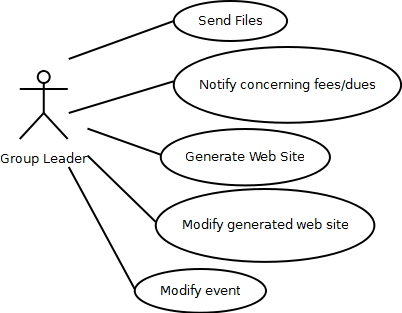
\includegraphics[width=5.5811in,height=4.3484in]{Gusspec-img2.png} 


\bigskip

\subsubsection[SYSTEM FEATURES]{\rmfamily SYSTEM FEATURES}
\subsubsection[System feature 1: Send Files]{\rmfamily System feature 1:
Send Files}
\begin{flushleft}
\tablehead{}
\begin{supertabular}{|m{6.42126in}|}
\hline
\bfseries\color{black} Use Case Description\\\hline
{\bfseries\color{black} Send Files}

{\color{black} Actors -- group leader }

{\color{black} Goals -- send file to many users}

{\color{black} Preconditions -- file has been uploaded to gus}

{\bfseries\color{black} Summary}

{\color{black} Related use cases:}

{\color{black} Send message}

{\bfseries\color{black} Steps}

\liststyleLi
\begin{enumerate}
\item \color{black} Click {\textquoteleft}Messages{\textquoteright}\item
\color{black} Click {\textquoteleft}New Message{\textquoteright}\item
\color{black} Click {\textquoteleft}Attach file{\textquoteright}\item
\color{black} On the dialog box, click {\textquoteleft}Send file from
gus{\textquoteright}\item \color{black} Select the file from the list
of files\item \color{black} Choose group members to send to\item
\color{black} Click send\end{enumerate}
~

{\color{black} Alternatives:}

\liststyleLii
\begin{enumerate}
\item \color{black} Include a message with the file\item \color{black}
Choose {\textquoteleft}send link to file{\textquoteright} option on
send dialog to send a link to a gus-hosted file instead of as an email
attachment\item \color{black} Upload the file from the send dialog
(option on button) instead of beforehand\end{enumerate}
\\\hline
\end{supertabular}
\end{flushleft}

\bigskip

\subsubsection[System feature 2: Notify concerning dues/fees]{\rmfamily
System feature 2: Notify concerning dues/fees}
\begin{flushleft}
\tablehead{}
\begin{supertabular}{|m{6.42126in}|}
\hline
\bfseries\color{black} Use Case Description\\\hline
{\bfseries\color{black} Notify concerning dues/fees}

{\color{black} Actors -- group leader}

{\color{black} Goals -- notify members of outstanding expenses}

{\color{black} Preconditions -- expense information is already entered
into gus}

{\bfseries\color{black} Summary}

{\color{black} Related use cases -- enter expense information, send
message}

{\bfseries\color{black} Steps}

\liststyleLiii
\begin{enumerate}
\item \color{black} Click {\textquoteleft}Money{\textquoteright}\item
\color{black} Click {\textquoteleft}Send notifications{\textquoteright}
(\textstyleDefaultParagraphFont{\textit{a dialog pops up}})\item
\color{black} Choose the users to be notified on the tree\item
\color{black} Click {\textquoteleft}Send{\textquoteright}
\ (\textstyleDefaultParagraphFont{\textit{the system sends out
emails}})\end{enumerate}
{\color{black} Alternatives}

\liststyleLiv
\begin{enumerate}
\item \color{black} Modify the message template to be sent\item
\color{black} Set up this task to recur automatically\end{enumerate}
\color{black} Postconditions -- a notification is emailed to each
applicable member\\\hline
\end{supertabular}
\end{flushleft}

\bigskip

\subsubsection[System feature 3: Generate web site]{\rmfamily System
feature 3: Generate web site}
\begin{flushleft}
\tablehead{}
\begin{supertabular}{|m{6.42126in}|}
\hline
\bfseries\color{black} Use Case Description\\\hline
{\bfseries\color{black} Generate web site}

{\color{black} Actors -- group leader}

{\color{black} Goals -- to generate a web site of information about a
group}

{\color{black} Preconditions -- gus is already set up to automatically
link to published pages}

{\bfseries\color{black} Summary}

{\color{black} Related use cases -- modify generated web site}

{\bfseries\color{black} Steps}

\liststyleLv
\begin{enumerate}
\item \color{black} Click {\textquoteleft}Web Site{\textquoteright}\item
\color{black} Click {\textquoteleft}Web site
options{\textquoteright}\item \color{black} Choose
members{\textquoteright} contact information to publish (usually the
group{\textquoteright}s senior members)\item \color{black} Leave the
box checked to publish the calendar\item \color{black} Type a group
description in the {\textquoteleft}group description{\textquoteright}
box\item \color{black} Click
{\textquoteleft}preview{\textquoteright}\item \color{black} Click
{\textquoteleft}publish{\textquoteright}\end{enumerate}
{\color{black} Alternatives -- uncheck the {\textquoteleft}publish
calendar{\textquoteright} box}

\color{black} Postconditions -- the website is published on the website,
and automatically linked to from its supergroup\\\hline
\end{supertabular}
\end{flushleft}

\bigskip

\subsubsection[System feature 4: Modify generated web site]{\rmfamily
System feature 4: Modify generated web site}
\begin{flushleft}
\tablehead{}
\begin{supertabular}{|m{6.42126in}|}
\hline
\bfseries\color{black} Use Case Description\\\hline
{\bfseries\color{black} Modify generated web site}

{\color{black} Actors -- group leader}

{\color{black} Goals -- to modify a generated web site of information
about a group}

{\color{black} Preconditions -- gus is already set up to automatically
link to published pages, a web site has already been published}

{\bfseries\color{black} Summary}

{\color{black} Related use cases -- generate web site}

{\bfseries\color{black} Steps}

\liststyleLvi
\begin{enumerate}
\item \color{black} Click {\textquoteleft}Web Site{\textquoteright}\item
\color{black} Click {\textquoteleft}Web site
options{\textquoteright}\item \color{black} Edit the settings on the
options page, including:\end{enumerate}
\liststyleLvii
\begin{enumerate}
\item \color{black} \ \ Publish calendar\item \color{black} \ \ Publish
contact information\item \color{black} \ \ Edit group description\item
\color{black} \ \ Edit/add group posts\end{enumerate}
\liststyleLvi
\begin{enumerate}
\item \color{black} Click {\textquoteleft}preview{\textquoteright}\item
\color{black} Click
{\textquoteleft}publish{\textquoteright}\end{enumerate}
~

{\color{black} Alternatives -- edit web site as desired}

\liststyleLii
\begin{enumerate}
\item \color{black} Postconditions -- the website is re-published on the
website with appropriate changes\end{enumerate}
\\\hline
\end{supertabular}
\end{flushleft}

\bigskip

\subsubsection[System feature 5: Modify Event]{\rmfamily System feature
5: Modify Event}
\begin{flushleft}
\tablehead{}
\begin{supertabular}{|m{6.42126in}|}
\hline
\bfseries\color{black} Use Case Description\\\hline
{\bfseries\color{black} Modify Event}

{\color{black} Actors -- group leader}

{\color{black} Goals -- modify (add, edit, remove) an event on the
calendar}

{\color{black} Preconditions - none}

{\bfseries\color{black} Summary}

{\color{black} Related use cases - none}

{\bfseries\color{black} Steps}

\liststyleLviii
\begin{enumerate}
\item \color{black} Click {\textquoteleft}Events{\textquoteright}\item
\color{black} Click {\textquoteleft}New event{\textquoteright}\item
\color{black} Add a title\item \color{black} Choose the date, time, and
recurrence\item \color{black} Check the {\textquoteleft}post to
site{\textquoteright} option\item \color{black} Check the
{\textquoteleft}email notifications to members{\textquoteright}
option\item \color{black} Modify the message to be sent\item
\color{black} Click {\textquoteleft}confirm
event{\textquoteright}\end{enumerate}
{\color{black} Alternatives }

\liststyleLix
\begin{enumerate}
\item \color{black} Choose not to publish on site\item \color{black}
Choose not to notify members via email\item \color{black} Send a custom
text message to members that have signed up for it\end{enumerate}
\color{black} Postconditions -- an event will be added to the calendar,
and the information will be sent as needed\\\hline
\end{supertabular}
\end{flushleft}

\bigskip


\bigskip


\bigskip


\bigskip


\bigskip


\bigskip


\bigskip


\bigskip


\bigskip


\bigskip


\bigskip


\bigskip


\bigskip


\bigskip


\bigskip


\bigskip


\bigskip


\bigskip


\bigskip


\bigskip


\bigskip


\bigskip


\bigskip

{\color{black}
\textstyleDefaultParagraphFont{\ (Sasha{\textquoteright}s use cases)}}


\bigskip

 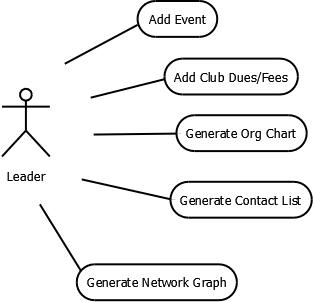
\includegraphics[width=3.9772in,height=3.8374in]{Gusspec-img3.png} 


\bigskip

\subsubsection[System feature 6: Add Event]{\rmfamily System feature 6:
Add Event}
\begin{flushleft}
\tablehead{}
\begin{supertabular}{|m{6.42126in}|}
\hline
\bfseries\color{black} Use Case Description\\\hline
{\bfseries\color{black} Add Event}

{\color{black} Actor - Leader}

{\color{black} Goal -- Add an event to fit leader specifications}

~

{\color{black} Precondition - Must be logged in as a leader.}

{\color{black} \textstyleDefaultParagraphFont{\textbf{Summary}}\newline
\textstyleDefaultParagraphFont{This task allows the leader to
}\textstyleDefaultParagraphFont{add}\textstyleDefaultParagraphFont{
}\textstyleDefaultParagraphFont{an event to the
group}\textstyleDefaultParagraphFont{{\textquoteright}}\textstyleDefaultParagraphFont{s
website.}}

~

{\color{black} Related use cases -- Modify event}

{\bfseries\color{black} Steps}

{\color{black} \ \ \ 1. Click
{\textquotedblleft}Events{\textquotedblright}}

{\color{black} \ \ \ 2. Click {\textquotedblleft}Add New
Event{\textquotedblright}}

{\color{black} \ \ \ 3. Complete event template as needed per desired
specifications}

{\color{black} \ \ \ 4. Click
{\textquotedblleft}Save{\textquotedblright}}

{\color{black} \ \ \ 5. Exit editing area by clicking on a different
navigational tab}

{\color{black} Alternatives -- }

{\color{black} At step 1, leader could click on a different navigational
tab to exit the {\textquotedblleft}Events{\textquotedblright}
area.\newline
At step 2, leader could click
{\textquotedblleft}Cancel{\textquotedblright} to exit the
{\textquotedblleft}Add New Event{\textquotedblright} area.}

\color{black} Postconditions -- Event has been added to fit
leader{\textquoteright}s specifications.\\\hline
\end{supertabular}
\end{flushleft}

\bigskip

\subsubsection[System feature 7: Add Club Dues/Fees]{\rmfamily System
feature 7: Add Club Dues/Fees}
\begin{flushleft}
\tablehead{}
\begin{supertabular}{|m{6.42126in}|}
\hline
\bfseries\color{black} Use Case Description\\\hline
{\bfseries\color{black} Add Club Dues/Fees}

{\color{black} Actors -- Leader, Server}

{\color{black} Goal -- Add new dues or fees to club members}

{\color{black} Precondition - Must be logged in as a leader, member(s)
must already exist.}

{\color{black} \textstyleDefaultParagraphFont{\textbf{Summary}}\newline
\textstyleDefaultParagraphFont{This task allows the leader to
}\textstyleDefaultParagraphFont{add club dues/fees to member(s).}}

~

{\color{black} Related use cases -- None}

{\bfseries\color{black} Steps}

{\color{black} \ \ \ 1. Click
{\textquotedblleft}Money{\textquotedblright} }

{\color{black} \ \ \ 2. Click {\textquotedblleft}Add
Fee{\textquotedblright} }

{\color{black} \ \ \ 3. Edit {\textquotedblleft}Name{\textquotedblright}
field and enter the name/reason for the fee/due.}

{\color{black} \ \ \ 4. Edit monetary amount section of template as
needed per desired specifications}

{\color{black} \ \ \ 5. Check member(s) for which the fee applies}

{\color{black} \ \ \ 6. Check frequency of fee (annual, monthly,
bi-weekly, one time, etc.)}

{\color{black} \ \ \ 7. Click
{\textquotedblleft}Add{\textquotedblright}}

{\color{black} \ \ \ 8. Upon receiving {\textquotedblleft}Add Fee
Request{\textquotedblright}, Server distributes a notification to all
applicable members (specified in Step 5). }

{\color{black} \ \ \ 8. Exit area by clicking on a different
navigational tab}

{\color{black} Alternatives -- }

{\color{black} At step 1, leader could click on a different navigational
tab to exit the {\textquotedblleft}Money{\textquotedblright}
area.\newline
At step 2, leader could click
{\textquotedblleft}Cancel{\textquotedblright} to exit the
{\textquotedblleft}Add Fee{\textquotedblright} area.}

\color{black} Postconditions -- A fee has been added to
member(s)\\\hline
\end{supertabular}
\end{flushleft}

\bigskip

\subsubsection[System feature 8: Generate Organization Chart]{\rmfamily
System feature 8: Generate Organization Chart}
\begin{flushleft}
\tablehead{}
\begin{supertabular}{|m{6.42126in}|}
\hline
\bfseries\color{black} Use Case Description\\\hline
{\bfseries\color{black} Generate Organizational Chart}

{\color{black} Actor - Leader}

{\color{black} Goal -- Generate an organizational chart of the group and
publish it to the group{\textquoteright}s website.}

{\color{black} Precondition -- Must be logged in as a leader, member(s)
must already exist.}

{\color{black} \textstyleDefaultParagraphFont{\textbf{Summary}}\newline
\textstyleDefaultParagraphFont{This }\textstyleDefaultParagraphFont{task
allows the leader to generate an organizational chart of the group and
publish it to the
group}\textstyleDefaultParagraphFont{{\textquoteright}}\textstyleDefaultParagraphFont{s
website.}}

~

{\color{black} Related use cases -- }

{\color{black} Send chart to members}

{\bfseries\color{black} Steps}

{\color{black} \ \ \ 1. Click
{\textquotedblleft}Website{\textquotedblright} }

{\color{black} \ \ \ 2. Click {\textquotedblleft}Generate Org
Chart{\textquotedblright} }

{\color{black} \ \ \ 3. Click
{\textquotedblleft}Publish{\textquotedblright}}

{\color{black} \ \ \ 4. Exit area by clicking on a different
navigational tab}

{\color{black} Alternatives -- }

{\color{black} At step 1, leader could click on a different navigational
tab to exit the {\textquotedblleft}Website{\textquotedblright}
area.\newline
At step 2, leader could click
{\textquotedblleft}Cancel{\textquotedblright} to stop generating the
chart.}

{\color{black} At step 2, leader could click {\textquotedblleft}Generate
Org Chart{\textquotedblright} to re-generate chart if chart did not
have desired outcome.}

\color{black} Postconditions -- An organizational chart has been added
to the group{\textquoteright}s website.\\\hline
\end{supertabular}
\end{flushleft}

\bigskip

\subsubsection[System feature 9: Generate Contact List]{\rmfamily System
feature 9: Generate Contact List}
\begin{flushleft}
\tablehead{}
\begin{supertabular}{|m{6.42126in}|}
\hline
\bfseries\color{black} Use Case Description\\\hline
{\bfseries\color{black} Generate Contact List}

{\color{black} Actor - Leader}

{\color{black} Goal -- Create a list of contact information of group
members}

{\color{black} Precondition - Must be logged in as a leader, member(s)
must already exist.}

{\color{black} \textstyleDefaultParagraphFont{\textbf{Summary}}\newline
\textstyleDefaultParagraphFont{This task allows the leader
}\textstyleDefaultParagraphFont{generate a contact list of all group
members}}

~

{\color{black} Related use cases -- }

{\color{black} Publish Contact List}

{\color{black} Send Contact List}

{\color{black} Save Contact List}

{\bfseries\color{black} Steps}

{\color{black} \ \ \ 1. Click
{\textquotedblleft}Group{\textquotedblright} }

{\color{black} \ \ \ 2. Click {\textquotedblleft}Contact
List{\textquotedblright} }

{\color{black} \ \ \ 3. Check members to be added to contact list
(default is all members)}

{\color{black} \ \ \ 4. Click
{\textquotedblleft}Generate{\textquotedblright}}

{\color{black} \ \ \ 5. Exit area by clicking on a different
navigational tab}

{\color{black} Alternatives -- }

{\color{black} At step 1, leader could click on a different navigational
tab to exit the {\textquotedblleft}Group{\textquotedblright}
area.\newline
At step 2 and 3, leader could click
{\textquotedblleft}Cancel{\textquotedblright} to exit the
{\textquotedblleft}Contact List{\textquotedblright} area.}

{\color{black} At step 4, leader could click
{\textquotedblleft}Cancel{\textquotedblright} to stop generation of
list}

\color{black} Postconditions -- A contact list has been
generated.\\\hline
\end{supertabular}
\end{flushleft}

\bigskip

\subsubsection[System feature 10: Generate Network Graph]{\rmfamily
System feature 10: Generate Network Graph}
\begin{flushleft}
\tablehead{}
\begin{supertabular}{|m{6.42126in}|}
\hline
\bfseries\color{black} Use Case Description\\\hline
{\bfseries\color{black} Generate Graphical Network}

{\color{black} Actor - Leader}

{\color{black} Goal -- Generate a network graph that displays
relationships between subgroups based on specific data provided and
display it on the group{\textquoteright}s website}

{\color{black} Precondition - Must be logged in as a leader.}

{\color{black} \textstyleDefaultParagraphFont{\textbf{Summary}}\newline
\textstyleDefaultParagraphFont{This task allows the leader
}\textstyleDefaultParagraphFont{generate a network graph and display it
on the
group}\textstyleDefaultParagraphFont{{\textquoteright}}\textstyleDefaultParagraphFont{s
website.}}

~

{\color{black} Related use cases -- None.}

{\color{black} \textstyleDefaultParagraphFont{\textbf{Steps}}}

{\color{black} \ \ \ 1. Click
{\textquotedblleft}Website{\textquotedblright} }

{\color{black} \ \ \ 2. Click {\textquotedblleft}Generate Network
Graph{\textquotedblright} }

{\color{black} \ \ \ 3. Check category option(s) under
{\textquotedblleft}Subcategory{\textquotedblright} (i.e. major,
membership numbers, etc)}

{\color{black} \ \ \ 4. Click
{\textquotedblleft}Publish{\textquotedblright}}

{\color{black} \ \ \ 5. Exit area by clicking on a different
navigational tab}

{\color{black} Alternatives -- }

{\color{black} At step 1, leader could click on a different navigational
tab to exit the {\textquotedblleft}Website{\textquotedblright}
area.\newline
At step 2 and 3, leader could click
{\textquotedblleft}Cancel{\textquotedblright} to exit the
{\textquotedblleft}Generate Network Graph{\textquotedblright} area.}

{\color{black} At step 3, leader could choose a different subcategory
option.}

{\color{black} At step 4, leader could click
{\textquotedblleft}Cancel{\textquotedblright} to stop generation of the
graph.}

\color{black} Postconditions -- A network graph has been published to
the group{\textquoteright}s website.\\\hline
\end{supertabular}
\end{flushleft}

\bigskip


\bigskip


\bigskip


\bigskip


\bigskip


\bigskip


\bigskip


\bigskip


\bigskip


\bigskip


\bigskip


\bigskip


\bigskip


\bigskip


\bigskip


\bigskip


\bigskip


\bigskip


\bigskip


\bigskip


\bigskip


\bigskip


\bigskip


\bigskip


\bigskip


\bigskip


\bigskip


\bigskip


\bigskip


\bigskip


\bigskip


\bigskip


\bigskip


\bigskip


\bigskip


\bigskip

{\color{black}
(Chandler{\textquoteright}s use cases)}

\subsubsection[System feature 11: Create user account]{\rmfamily System
feature 11: Create user account}
\begin{flushleft}
\tablehead{}
\begin{supertabular}{|m{3.17056in}|}
\hline
\liststyleLFOxiii
\begin{enumerate}
\item \sffamily\bfseries\color{black} Use Case
Description\end{enumerate}
\\\hline
\liststyleLFOxiii
\setcounter{saveenum}{\value{enumi}}
\begin{enumerate}
\setcounter{enumi}{\value{saveenum}}
\item \sffamily\color{black}
\textstyleDefaultParagraphFont{\textbf{Name:
}}\textstyleDefaultParagraphFont{Create user account}\item
\sffamily\color{black} \textstyleDefaultParagraphFont{\textbf{Actors:
}}\textstyleDefaultParagraphFont{New User}\item \sffamily\color{black}
\textstyleDefaultParagraphFont{\textbf{Goals:
}}\textstyleDefaultParagraphFont{Create new account}\item
\sffamily\color{black}
\textstyleDefaultParagraphFont{\textbf{Preconditions:
}}\textstyleDefaultParagraphFont{Account does not already exist.}\item
\sffamily\bfseries\color{black} Steps: \item \sffamily\color{black}
\textstyleDefaultParagraphFont{Select {\textquotedblleft}sign
up{\textquotedblright} from application}\item \sffamily\color{black}
\textstyleDefaultParagraphFont{Enter email address and name}\item
\sffamily\color{black} \textstyleDefaultParagraphFont{Enter
Password}\item \sffamily\color{black}
\textstyleDefaultParagraphFont{Select
{\textquotedblleft}finish{\textquotedblright}}\item
\sffamily\bfseries\color{black} Alternatives: \item
\sffamily\color{black} \textstyleDefaultParagraphFont{Email address
already registered}\item \sffamily\color{black}
\textstyleDefaultParagraphFont{Enter new email address}\item
\sffamily\color{black} \textstyleDefaultParagraphFont{Select
{\textquotedblleft}finish{\textquotedblright}}\item
\sffamily\bfseries\color{black} Postconditions: \item
\sffamily\color{black} \textstyleDefaultParagraphFont{Blank account is
created \ }\item ~
\item ~
\end{enumerate}
\\
\liststyleLFOxiii
\setcounter{saveenum}{\value{enumi}}
\begin{enumerate}
\setcounter{enumi}{\value{saveenum}}
\item ~
\end{enumerate}
\\\hline
\end{supertabular}
\end{flushleft}

\bigskip

\subsubsection[System feature 12: Create new group]{\rmfamily System
feature 12: Create new group}
\begin{flushleft}
\tablehead{}
\begin{supertabular}{|m{3.17056in}|}
\hline
\liststyleLFOxiii
\setcounter{saveenum}{\value{enumi}}
\begin{enumerate}
\setcounter{enumi}{\value{saveenum}}
\item \sffamily\bfseries\color{black} Use Case
Description\end{enumerate}
\\\hline
\liststyleLFOxiii
\setcounter{saveenum}{\value{enumi}}
\begin{enumerate}
\setcounter{enumi}{\value{saveenum}}
\item \sffamily\color{black}
\textstyleDefaultParagraphFont{\textbf{Name:
}}\textstyleDefaultParagraphFont{Create new group}\item
\sffamily\color{black} \textstyleDefaultParagraphFont{\textbf{Actors:
}}\textstyleDefaultParagraphFont{Existing user}\item
\sffamily\color{black} \textstyleDefaultParagraphFont{\textbf{Goals:
}}\textstyleDefaultParagraphFont{Create new account}\item
\sffamily\bfseries\color{black} Preconditions: \item
\sffamily\color{black} \textstyleDefaultParagraphFont{User has an
account}\item \sffamily\color{black}
\textstyleDefaultParagraphFont{Group by the same name does not already
exist}\item \sffamily\color{black} \textstyleDefaultParagraphFont{User
has appropriate privileges to create group in specified
location}\end{enumerate}
{\sffamily\bfseries\color{black} Steps: }

\liststyleLFOxiii
\setcounter{saveenum}{\value{enumi}}
\begin{enumerate}
\setcounter{enumi}{\value{saveenum}}
\item \sffamily\color{black} select {\textquotedbl}create new
group{\textquotedbl}\item \sffamily\color{black} specify group
name\item \sffamily\color{black} specify group administrator(s)\item
\sffamily\color{black} \textstyleDefaultParagraphFont{select
finish}\item \sffamily\bfseries\color{black} Alternatives: \item
\sffamily\color{black} select users to invite to group\item
\sffamily\color{black} \textstyleDefaultParagraphFont{select template
to preconfigure group settings}\item \sffamily\bfseries\color{black}
Postconditions: \item \sffamily\color{black}
\textstyleDefaultParagraphFont{New group is created}\item ~
\item ~
\end{enumerate}
\\\hline
\end{supertabular}
\end{flushleft}

\bigskip

\subsubsection[System feature 13: Delete user account]{\rmfamily System
feature 13: Delete user account}
\begin{flushleft}
\tablehead{}
\begin{supertabular}{|m{3.17056in}|}
\hline
\liststyleLFOxiii
\setcounter{saveenum}{\value{enumi}}
\begin{enumerate}
\setcounter{enumi}{\value{saveenum}}
\item \sffamily\bfseries\color{black} Use Case
Description\end{enumerate}
\\\hline
\liststyleLFOxiii
\setcounter{saveenum}{\value{enumi}}
\begin{enumerate}
\setcounter{enumi}{\value{saveenum}}
\item \sffamily\color{black}
\textstyleDefaultParagraphFont{\textbf{Name:
}}\textstyleDefaultParagraphFont{Delete user account}\item
\sffamily\color{black} \textstyleDefaultParagraphFont{\textbf{Actors:
}}\textstyleDefaultParagraphFont{Existing user}\item
\sffamily\color{black} \textstyleDefaultParagraphFont{\textbf{Goals:
}}\textstyleDefaultParagraphFont{permanently delete account}\item
\sffamily\bfseries\color{black} Preconditions: \end{enumerate}
{\sffamily\color{black} User has an account.}

\liststyleLFOxiii
\setcounter{saveenum}{\value{enumi}}
\begin{enumerate}
\setcounter{enumi}{\value{saveenum}}
\item \sffamily\bfseries\color{black} Summary\item
\sffamily\color{black} User account will be permanently
removed.\end{enumerate}
{\sffamily\bfseries\color{black} Steps: }

\liststyleLFOxiii
\setcounter{saveenum}{\value{enumi}}
\begin{enumerate}
\setcounter{enumi}{\value{saveenum}}
\item \sffamily\color{black} Select {\textquotedbl}delete
account{\textquotedbl}\item \sffamily\color{black}
\textstyleDefaultParagraphFont{Acknowledge warning {\textquotedbl}all
groups administered by you and without another administrator will be
deleted.{\textquotedbl}}\item \sffamily\bfseries\color{black}
Alternatives: \item \sffamily\color{black}
\textstyleDefaultParagraphFont{C}\textstyleDefaultParagraphFont{ancel
account deletion at warning.}\item \sffamily\bfseries\color{black}
Postconditions: \end{enumerate}
{\sffamily\color{black} User account no longer exists}

\liststyleLFOxiii
\setcounter{saveenum}{\value{enumi}}
\begin{enumerate}
\setcounter{enumi}{\value{saveenum}}
\item ~
\item ~
\end{enumerate}
\\\hline
\end{supertabular}
\end{flushleft}

\bigskip

\subsubsection[System feature 14: Delete old group]{\rmfamily System
feature 14: Delete old group}
\begin{flushleft}
\tablehead{}
\begin{supertabular}{|m{3.17056in}|}
\hline
\liststyleLFOxiii
\setcounter{saveenum}{\value{enumi}}
\begin{enumerate}
\setcounter{enumi}{\value{saveenum}}
\item \sffamily\bfseries\color{black} Use Case
Description\end{enumerate}
\\\hline
\liststyleLFOxiii
\setcounter{saveenum}{\value{enumi}}
\begin{enumerate}
\setcounter{enumi}{\value{saveenum}}
\item \sffamily\color{black}
\textstyleDefaultParagraphFont{\textbf{Name:
}}\textstyleDefaultParagraphFont{Delete old group}\item
\sffamily\color{black} \textstyleDefaultParagraphFont{\textbf{Actors:
}}\textstyleDefaultParagraphFont{Existing user}\item
\sffamily\color{black} \textstyleDefaultParagraphFont{\textbf{Goals:
}}\textstyleDefaultParagraphFont{permanently delete group}\item
\sffamily\bfseries\color{black} Preconditions: \item
\sffamily\color{black} \textstyleDefaultParagraphFont{User is a group
administrator.}\item \sffamily\bfseries\color{black}
Summary\end{enumerate}
{\sffamily\color{black} Group will be permanently removed.}

{\sffamily\bfseries\color{black} Steps: }

\liststyleLFOxiii
\setcounter{saveenum}{\value{enumi}}
\begin{enumerate}
\setcounter{enumi}{\value{saveenum}}
\item \sffamily\color{black} Select {\textquotedbl}delete
group{\textquotedbl}\item \sffamily\color{black}
\textstyleDefaultParagraphFont{Acknowledge warning {\textquotedbl}all
groups administered by you and without another administrator will be
deleted.{\textquotedbl}}\item \sffamily\bfseries\color{black}
Alternatives: \item \sffamily\color{black}
\textstyleDefaultParagraphFont{C}\textstyleDefaultParagraphFont{ancel
}\textstyleDefaultParagraphFont{group deletion
}\textstyleDefaultParagraphFont{at warning.}\item
\sffamily\bfseries\color{black} Postconditions: \end{enumerate}
{\sffamily\color{black} Group no longer exists.}

\liststyleLFOxiii
\setcounter{saveenum}{\value{enumi}}
\begin{enumerate}
\setcounter{enumi}{\value{saveenum}}
\item ~
\item ~
\end{enumerate}
\\\hline
\end{supertabular}
\end{flushleft}

\bigskip

\subsubsection[System feature 15: Change group permissions]{\rmfamily
System feature 15: Change group permissions}
\begin{flushleft}
\tablehead{}
\begin{supertabular}{|m{3.17056in}|}
\hline
\liststyleLFOxiii
\setcounter{saveenum}{\value{enumi}}
\begin{enumerate}
\setcounter{enumi}{\value{saveenum}}
\item \sffamily\bfseries\color{black} Use Case
Description\end{enumerate}
\\\hline
\liststyleLFOxiii
\setcounter{saveenum}{\value{enumi}}
\begin{enumerate}
\setcounter{enumi}{\value{saveenum}}
\item \sffamily\color{black}
\textstyleDefaultParagraphFont{\textbf{Name:
}}\textstyleDefaultParagraphFont{Change
}\textstyleDefaultParagraphFont{group permissions. }\item
\sffamily\color{black} \textstyleDefaultParagraphFont{\textbf{Actors:
}}\textstyleDefaultParagraphFont{Existing user}\item
\sffamily\bfseries\color{black} Preconditions: \item
\sffamily\color{black} \textstyleDefaultParagraphFont{User is a group
administrator.}\item \sffamily\bfseries\color{black}
Summary\end{enumerate}
{\sffamily\color{black} Specify which users have certain permissions in
the group.}

{\sffamily\bfseries\color{black} Steps: }

\liststyleLFOxiii
\setcounter{saveenum}{\value{enumi}}
\begin{enumerate}
\setcounter{enumi}{\value{saveenum}}
\item \sffamily\color{black} \textstyleDefaultParagraphFont{Select
desired group}\item \sffamily\color{black}
\textstyleDefaultParagraphFont{Select {\textquotedblleft}group
permissions{\textquotedblright}}\item \sffamily\color{black}
\textstyleDefaultParagraphFont{Select desired user}\item
\sffamily\color{black} \textstyleDefaultParagraphFont{Check or uncheck
desired permissions}\item \sffamily\bfseries\color{black}
Postconditions: \end{enumerate}
{\sffamily\color{black} Permissions are changed.}

\liststyleLFOxiii
\setcounter{saveenum}{\value{enumi}}
\begin{enumerate}
\setcounter{enumi}{\value{saveenum}}
\item ~
\item ~
\end{enumerate}
\\\hline
\end{supertabular}
\end{flushleft}

\bigskip


\bigskip


\bigskip


\bigskip


\bigskip


\bigskip

{\color{black}
(Leah{\textquoteright}s use cases)}

 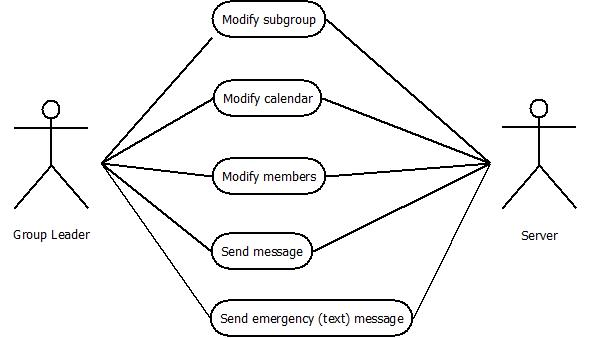
\includegraphics[width=6.1516in,height=3.5228in]{Gusspec-img4.jpg} 

\subsubsection[System feature 16: Modify Subgroup]{\rmfamily System
feature 16: Modify Subgroup}
\begin{flushleft}
\tablehead{}
\begin{supertabular}{|m{4.98376in}|}
\hline
\bfseries\color{black} Use Case Description\\\hline
{\bfseries\color{black} Name: Modify Subgroup}

{\color{black} Actors: Group Leader}

{\color{black} Goals: Create, remove or rename a subgroup}

{\bfseries\color{black} Summary: }

{\color{black} This function is used to create, rename, or delete groups
under a group that you already control.}

{\color{black} \textstyleDefaultParagraphFont{\textbf{Preconditions:
}}none}

{\bfseries\color{black} Steps}

{\color{black} \ \ \ 1. Ask user which subgroup they would like to
modify}

{\color{black} \ \ \ 2. Check with server to see if the subgroup already
exists}

{\color{black} \ \ \ 3. Ask questions to determine which action to take}

{\color{black} \ \ \ 4. Perform desired action}

{\color{black} \ \ \ 5. If a task has been performed, inform the user of
what they did.}

{\bfseries\color{black} Alternatives}

{\color{black} \ \ \ At step 3 the group leader may choose to rename,
remove, or create a subgroup based on whether the group already exists
or not determined in step 2. The group leader may also cancel the
action at this time.}

~
\\\hline
\end{supertabular}
\end{flushleft}

\bigskip

\subsubsection[System feature \ 17: Modify Calendar]{\rmfamily System
feature \ 17: Modify Calendar}
\begin{flushleft}
\tablehead{}
\begin{supertabular}{|m{4.98376in}|}
\hline
\bfseries\color{black} Use Case Description\\\hline
{\color{black} \textstyleDefaultParagraphFont{\textbf{Name:
}}\textstyleDefaultParagraphFont{\textsf{\textbf{Modify calendar}}}}

{\color{black} Actors: Group Leader}

{\color{black} Goals: Create, remove, or change the properties of a
calendar event.}

{\color{black} Preconditions: None}

{\bfseries\color{black} Summary}

{\color{black} This function is used to create, change, or delete
calendar events for a group that you control.}

{\bfseries\color{black} Steps}

{\color{black} \ \ \ 1. Ask user which calendar event they would like to
modify}

{\color{black} \ \ \ 2. Check to see if the event already exists}

{\color{black} \ \ \ 3. Ask if they would like to create, change, or
remove an event.}

{\color{black} \ \ \ 4. Perform desired action}

{\color{black} \ \ \ 5. If a task has been performed, inform the user of
what they did.}

{\bfseries\color{black} Alternatives}

{\color{black} \textstyleDefaultParagraphFont{\textbf{\ \ \ }}From step
2:}

{\color{black} \ \ \ 3. If it exists, ask if they would like to change
or remove it.}

{\color{black} \ \ \ \ \ \ a. if remove, remove it.}

{\color{black} \ \ \ \ \ \ b. if change, bring up a window form for the
actor to input new values into.}

{\color{black} \ \ \ 4. If it doesn{\textquoteright}t exist, ask if they
would like to create it.}

\color{black} \ \ \ The user also has the option to cancel action during
step 3\\\hline
\end{supertabular}
\end{flushleft}

\bigskip


\bigskip

\subsubsection[System feature 18: Modify Members]{\rmfamily System
feature 18: Modify Members}
\begin{flushleft}
\tablehead{}
\begin{supertabular}{|m{6.42126in}|}
\hline
\bfseries\color{black} Use Case Description\\\hline
{\color{black} \textstyleDefaultParagraphFont{\textbf{Name:
}}\textstyleDefaultParagraphFont{\textsf{\textbf{Modify
}}}\textstyleDefaultParagraphFont{\textsf{\textbf{members}}}}

{\color{black} Actors: Group Leader}

{\color{black} Goals: Add or remove a member from a group. Or appoint
someone to be the leader of a group.}

{\color{black} \textstyleDefaultParagraphFont{\textbf{Preconditions:
}}none}

{\bfseries\color{black} Summary}

{\color{black} This function is used to add, change privileges of or
delete a member in a group that you control.}

~

{\bfseries\color{black} Steps}

\liststyleLx
\begin{enumerate}
\item \color{black} Ask user if they would like to add a member, remove
a member, or appoint a member as a leader.\item \color{black} Ask which
group to apply changes to\end{enumerate}
{\color{black} \ \ \ 3. Add a member}

{\color{black} \ \ \ \ \ \ a. ask who to add}

{\color{black} \ \ \ \ \ \ b. look up who to add}

{\color{black} \ \ \ \ \ \ c. if no matching information previously in
the system, ask for as much information as possible. Alternatively, try
to retrieve the info from an online directory (such as that provided by
many universities such as the U of I).}

{\color{black} \ \ \ \ \ \ d. add the member to the group}

{\color{black} \ \ \ 4. If a task has been performed, inform the user of
what they did.}

{\bfseries\color{black} Alternatives}

{\color{black} \textstyleDefaultParagraphFont{\textbf{\ \ \ }}Alternate
step 3, depending on the user reply to the question asked in step 1}

{\color{black} \ \ \ 3. remove a member}

{\color{black} \ \ \ \ \ \ a. check to see if they really are a member}

{\color{black} \ \ \ \ \ \ b. if so, ask for confirmation}

{\color{black} \ \ \ \ \ \ c. upon receiving confirmation, remove the
member from the group.}

{\color{black} \ \ \ 3. If making a member a leader:}

{\color{black} \ \ \ \ \ \ a. check to see if they are already a member}

{\color{black} \ \ \ \ \ \ b. if not, add them as a member}

{\color{black} \ \ \ \ \ \ c. ask for confirmation}

\color{black} \ \ \ \ \ \ d. upon receiving confirmation, change the
status to group leader\\\hline
\end{supertabular}
\end{flushleft}

\bigskip

\subsubsection[System feature 19: Send E{}-Mail]{\rmfamily System
feature 19: Send E-Mail}
\begin{flushleft}
\tablehead{}
\begin{supertabular}{|m{6.42126in}|}
\hline
\bfseries\color{black} Use Case Description\\\hline
{\color{black} \textstyleDefaultParagraphFont{\textbf{Name:
}}\textstyleDefaultParagraphFont{\textsf{\textbf{Send Email}}}}

{\color{black} Actors: Group Leader}

{\color{black} Goals: send email to all members of a group or selective
members of a group.}

~

{\color{black} \textstyleDefaultParagraphFont{\textbf{Preconditions:}}
The people who the group leader would like to email are part of his/her
subgroup, or a subgroup of his/her subgroup.}

~

{\bfseries\color{black} Summary}

{\color{black} This function is used to send a message to selected
members of a group.}

~

{\bfseries\color{black} Steps}

{\color{black} \ \ \ 1. Get user to type email}

{\color{black} \ \ \ 2. Ask user to select who to send the mail to. }

{\color{black} \ \ \ 3. pop up a check list of members along with
buttons for {\textquotedblleft}everyone{\textquotedblright}
{\textquotedblleft}and everyone including me{\textquotedblright}}

{\color{black} \ \ \ 4. User pushes send button}

{\color{black} \ \ \ 5.Send email to those members whose boxes have been
selected}

{\color{black} \ \ \ 6. If a task has been performed, inform the user of
what they did.}

{\bfseries\color{black} Alternatives}

\color{black} \ \ \ The user may cancel at step 1, 3, or 4 by clicking a
button labeled {\textquotedblleft}cancel{\textquotedblright}\\\hline
\end{supertabular}
\end{flushleft}

\bigskip


\bigskip


\bigskip


\bigskip


\bigskip


\bigskip


\bigskip

\subsubsection[System feature 20: Send Emergency (text)
Message]{\rmfamily System feature 20: Send Emergency (text) Message}
\begin{flushleft}
\tablehead{}
\begin{supertabular}{|m{6.42126in}|}
\hline
\bfseries\color{black} Use Case Description\\\hline
{\color{black} \textstyleDefaultParagraphFont{\textbf{Name:
}}\textstyleDefaultParagraphFont{\textsf{\textbf{Send Emergency (text)
Message}}}}

{\color{black} Actors: Group Leader}

{\color{black} Goals: Create, remove, or change the properties of a
calendar event.}

~

{\bfseries\color{black} Preconditions:}

{\color{black} The people who the group leader would like to send an
emergency/high importance message to are part of his/her subgroup, or a
subgroup of his/her subgroup.}

~

{\bfseries\color{black} Summary}

{\color{black} This function is used to send an emergency/ high
importance message to selected members of a group.}

~

{\bfseries\color{black} Steps}

{\color{black} \ \ \ 1. Bring up a form where the user will type the
email}

{\color{black} \ \ \ 2. Ask user to select who to send the mail to. }

{\color{black} \ \ \ 3. pop up a check list of members along with
buttons for {\textquotedblleft}everyone{\textquotedblright}
{\textquotedblleft}and everyone including me{\textquotedblright}}

{\color{black} \ \ \ 4. User pushes send button}

{\color{black} \ \ \ 5.Send text to those members who{\textquoteright}s
boxes have been selected and who have opted in to receiving texts}

{\color{black} \ \ \ 6. Send email to those members whose boxes have
been selected and who have not opted in to receiving texts.}

{\color{black} \ \ \ 7. If a task has been performed, inform the user of
what they did.}

{\bfseries\color{black} Alternatives}

\color{black} \ \ \ The user may cancel at step 1, 3, or 4 by clicking a
button labeled {\textquotedblleft}cancel{\textquotedblright}\\\hline
\end{supertabular}
\end{flushleft}

\bigskip


\bigskip


\bigskip


\bigskip

{\color{black}
(John{\textquoteright}s use cases)}


\bigskip


\bigskip

\subsubsection[System feature 21: Search Groups]{\rmfamily System
feature 21: Search Groups}
\begin{flushleft}
\tablehead{}
\begin{supertabular}{|m{3.17056in}|m{3.1712599in}|}
\hline
\bfseries\color{black} Use Case Description &
\paragraph[Non{}-task feature
description]{\selectlanguage{english}\rmfamily Non-task feature
description}
\\\hline
{\bfseries\color{black} Search Groups}

{\color{black} Actor - Member}

{\color{black} Goal -- Generate a list of groups based on search
keywords and other search conditions.}

{\color{black} Precondition - Must be logged in as a member.}

{\color{black} \textstyleDefaultParagraphFont{\textbf{Summary}}\newline
\textstyleDefaultParagraphFont{This task allows a member to search
through the various groups (sub-organizational units) present within
the application.}}

~

{\color{black} Related use cases -- \#22: {\textquotedblleft}Select
Criteria to View Group Suggestions{\textquotedblright}.}

{\color{black} \textstyleDefaultParagraphFont{\textbf{Steps}}}

{\color{black} \ \ \ 1. Click
{\textquotedblleft}Groups{\textquotedblright} }

{\color{black} \ \ \ 2. Click
{\textquotedblleft}Search{\textquotedblright} }

{\color{black} \ \ \ 3. Enter search criteria.}

{\color{black} \ \ \ 4. Click
{\textquotedblleft}Search{\textquotedblright}}

{\color{black} \ \ \ 5. Groups appear as clickable links}

{\color{black} Alternatives -- }

\color{black} This could be implemented as part of a site-wide search,
making steps 1 and possibly 2 irrelevant.\newline
Postconditions -- A list of groups related to the criteria has been
given. &
\paragraph[\ Introduction/Purpose of this
feature]{\selectlanguage{english}\rmfamily \ Introduction/Purpose of
this feature}
{\color{black} The purpose is for a member to find groups based on
specific criteria in order to observe the group page and/or join the
group.}

\paragraph[Input/Output sequence for this
feature]{\selectlanguage{english}\rmfamily Input/Output sequence for
this feature}
{\color{black} Takes place in the GUI.}

\paragraph[Design constraints of this
feature]{\selectlanguage{english}\rmfamily Design constraints of this
feature}
{\color{black} HTML preview must be supported.}

\paragraph[Performance requirements of this
feature]{\selectlanguage{english}\rmfamily Performance requirements of
this feature}
{\color{black} Results of completing task should be visible
immediately.}

\paragraph[Detailed functional requirements of this
feature]{\selectlanguage{english}\rmfamily Detailed functional
requirements of this feature}
\subparagraph[Functional requirement 1.1]{\selectlanguage{english}
Functional requirement 1.1}
{\color{black} Gus must be able to locate needed data in the database
and assemble appropriately.}

\subparagraph[Functional requirement 1.2]{\selectlanguage{english}
Functional requirement 1.2}
{\color{black} Gus must be able to update data in a timely manner so as
to be transparent to the member.}

~
\\\hline
\end{supertabular}
\end{flushleft}
\subsubsection[System feature 22: Select Criteria to View Group
Suggestions]{\rmfamily System feature 22: Select Criteria to View Group
Suggestions}
\begin{flushleft}
\tablehead{}
\begin{supertabular}{|m{3.17056in}|m{3.1712599in}|}
\hline
\bfseries\color{black} Use Case Description &
\paragraph[Non{}-task feature
description]{\selectlanguage{english}\rmfamily Non-task feature
description}
\\\hline
{\bfseries\color{black} Search Groups}

{\color{black} Actor - Member}

{\color{black} Goal -- Generate a list of groups based on major,
membership numbers, and any number of other categories.}

{\color{black}
\textstyleDefaultParagraphFont{\textbf{Summary}}\textstyleDefaultParagraphFont{\textbf{\ \ }}\newline
\textstyleDefaultParagraphFont{This task allows a member to search
through the various groups (sub-organizational units) present within
the application.}}

~

{\color{black} Related use cases -- \#21: {\textquotedblleft}Search
Groups{\textquotedblright}.}

{\color{black} \textstyleDefaultParagraphFont{\textbf{Steps}}}

{\color{black} \ \ \ 1. Click
{\textquotedblleft}Groups{\textquotedblright} }

{\color{black} \ \ \ 2. Click
{\textquotedblleft}Search{\textquotedblright} }

{\color{black} \ \ \ 3. Enter search criteria.}

{\color{black} \ \ \ 4. Click
{\textquotedblleft}Search{\textquotedblright}}

{\color{black} \ \ \ 5. Groups appear as clickable links}

{\color{black} Alternatives -- }

\color{black} This could be implemented as part of a site-wide search,
making steps 1 and possibly 2 irrelevant.\newline
Postconditions -- A list of groups related to the criteria has been
given. &
\paragraph[\ Introduction/Purpose of this
feature]{\selectlanguage{english}\rmfamily \ Introduction/Purpose of
this feature}
{\color{black} The purpose is for a member to find groups based on
specific criteria in order to observe the group page and/or join the
group.}

\paragraph[Input/Output sequence for this
feature]{\selectlanguage{english}\rmfamily Input/Output sequence for
this feature}
{\color{black} Takes place in the GUI.}

\paragraph[Design constraints of this
feature]{\selectlanguage{english}\rmfamily Design constraints of this
feature}
{\color{black} HTML preview must be supported.}

\paragraph[Performance requirements of this
feature]{\selectlanguage{english}\rmfamily Performance requirements of
this feature}
{\color{black} Results of completing task should be visible
immediately.}

\paragraph[Detailed functional requirements of this
feature]{\selectlanguage{english}\rmfamily Detailed functional
requirements of this feature}
\subparagraph[Functional requirement 1.1]{\selectlanguage{english}
Functional requirement 1.1}
{\color{black} Gus must be able to locate needed data in the database
and assemble appropriately.}

\subparagraph[Functional requirement 1.2]{\selectlanguage{english}
Functional requirement 1.2}
{\color{black} Gus must be able to update data in a timely manner so as
to be transparent to the member.}

~
\\\hline
\end{supertabular}
\end{flushleft}

\bigskip

\subsubsection[System feature 23: Download/Upload Calendar
File]{\rmfamily System feature 23: Download/Upload Calendar File}
\begin{flushleft}
\tablehead{}
\begin{supertabular}{|m{3.17056in}|m{3.1712599in}|}
\hline
\bfseries\color{black} Use Case Description &
\paragraph[Non{}-task feature
description]{\selectlanguage{english}\rmfamily Non-task feature
description}
\\\hline
{\bfseries\color{black} Search Groups}

{\color{black} Actor - Member}

{\color{black} Goal -- Allow a member to download or upload a calendar
file in the standard iCal format (which is compatible with most other
online and desktop services).}

{\color{black}
\textstyleDefaultParagraphFont{\textbf{Summary}}\textstyleDefaultParagraphFont{\textbf{\ \ }}\newline
\textstyleDefaultParagraphFont{This task allows a member to download a
particular calendar as a file or upload and optionally merge a calendar
file from the member{\textquoteright}s computer.}}

~

{\color{black} Related use cases -- \#28: {\textquotedblleft}Download
composite calendar of all groups user is member of{\textquotedblright},
\#7: {\textquotedblleft}Modify Calendar{\textquotedblright}.}

{\color{black} \textstyleDefaultParagraphFont{\textbf{Steps}}}

{\color{black} \ \ \ 1. Click
{\textquotedblleft}Calendar{\textquotedblright} }

{\color{black} \ \ \ 2. Click
{\textquotedblleft}Download/Upload{\textquotedblright} }

{\color{black} \ \ \ 3. Choose a calendar to download OR choose a file
to upload.}

{\color{black} \ \ \ 4. Click
{\textquotedblleft}Download{\textquotedblright} or
{\textquotedblleft}Upload{\textquotedblright} (whichever is relevant)}

{\color{black} \ \ \ 5. Uploaded calendar is shown (if uploaded), or a
{\textquotedblleft}finished{\textquotedblright} message is shown.}

{\color{black} Alternatives -- }

\color{black} Step 1 may occur after other steps depending on calendar
location on site.\newline
Postconditions -- A calendar has been downloaded or uploaded. &
\paragraph[\ Introduction/Purpose of this
feature]{\selectlanguage{english}\rmfamily \ Introduction/Purpose of
this feature}
{\color{black} The purpose is for a member to upload and download
calendars to and from the member{\textquoteright}s computer.}

\paragraph[Input/Output sequence for this
feature]{\selectlanguage{english}\rmfamily Input/Output sequence for
this feature}
{\color{black} Takes place in the GUI.}

\paragraph[Design constraints of this
feature]{\selectlanguage{english}\rmfamily Design constraints of this
feature}
{\color{black} HTML preview must be supported.}

\paragraph[Performance requirements of this
feature]{\selectlanguage{english}\rmfamily Performance requirements of
this feature}
{\color{black} Results of completing task should be visible
immediately.}

\paragraph[Detailed functional requirements of this
feature]{\selectlanguage{english}\rmfamily Detailed functional
requirements of this feature}
\subparagraph[Functional requirement 1.1]{\selectlanguage{english}
Functional requirement 1.1}
{\color{black} Gus must be able to locate needed data in the database
and assemble appropriately.}

\subparagraph[Functional requirement 1.2]{\selectlanguage{english}
Functional requirement 1.2}
{\color{black} Gus must be able to update data in a timely manner so as
to be transparent to the member.}

~
\\\hline
\end{supertabular}
\end{flushleft}

\bigskip


\bigskip

\subsubsection[System feature 24: Log In]{\rmfamily System feature 24:
Log In}
\begin{flushleft}
\tablehead{}
\begin{supertabular}{|m{3.17056in}|m{3.1712599in}|}
\hline
\bfseries\color{black} Use Case Description &
\paragraph[Non{}-task feature
description]{\selectlanguage{english}\rmfamily Non-task feature
description}
\\\hline
{\bfseries\color{black} Search Groups}

{\color{black} Actor - User}

{\color{black} Goal -- Allow a member to log into the site as a member.}

{\color{black}
\textstyleDefaultParagraphFont{\textbf{Summary}}\textstyleDefaultParagraphFont{\textbf{\ \ }}\newline
\textstyleDefaultParagraphFont{This task allows a user to log in and
verify his or her identity on the website, thus becoming additional
types of Actors (for example, Member or Admin).}}

~

{\color{black} Related use cases -- None.}

{\color{black} \textstyleDefaultParagraphFont{\textbf{Steps}}}

{\color{black} \ \ \ 1. Click {\textquotedblleft}Log
In{\textquotedblright} menu option }

{\color{black} \ \ \ 2. Enter username.}

{\color{black} \ \ \ 3. Enter password.}

{\color{black} \ \ \ 4. Click {\textquotedblleft}Log
In{\textquotedblright}}

{\color{black} \ \ \ 5. Repeat or leave upon failure, or redirect to
homepage on success.}

{\color{black} Alternatives -- }

{\color{black} A {\textquotedblleft}success{\textquotedblright} message
may be displayed in place of an immediate redirection.}

\color{black} Postconditions -- The member has been authenticated on the
system. &
\paragraph[\ Introduction/Purpose of this
feature]{\selectlanguage{english}\rmfamily \ Introduction/Purpose of
this feature}
{\color{black} The purpose is for a member to authenticate himself or
herself on the system.}

\paragraph[Input/Output sequence for this
feature]{\selectlanguage{english}\rmfamily Input/Output sequence for
this feature}
{\color{black} Takes place in the GUI.}

\paragraph[Design constraints of this
feature]{\selectlanguage{english}\rmfamily Design constraints of this
feature}
{\color{black} HTML preview must be supported.}

\paragraph[Performance requirements of this
feature]{\selectlanguage{english}\rmfamily Performance requirements of
this feature}
{\color{black} Results of completing task should be visible
immediately.}

\paragraph[Detailed functional requirements of this
feature]{\selectlanguage{english}\rmfamily Detailed functional
requirements of this feature}
\subparagraph[Functional requirement 1.1]{\selectlanguage{english}
Functional requirement 1.1}
{\color{black} Gus must be able to locate needed data in the database
and assemble appropriately.}

\subparagraph[Functional requirement 1.2]{\selectlanguage{english}
Functional requirement 1.2}
{\color{black} Gus must be able to update data in a timely manner so as
to be transparent to the member.}

~
\\\hline
\end{supertabular}
\end{flushleft}

\bigskip

\subsubsection[System feature 25: Update e{}-mail address]{\rmfamily
System feature 25: Update e-mail address}
\begin{flushleft}
\tablehead{}
\begin{supertabular}{|m{3.17056in}|m{3.1712599in}|}
\hline
\bfseries\color{black} Use Case Description &
\paragraph[Non{}-task feature
description]{\selectlanguage{english}\rmfamily Non-task feature
description}
\\\hline
{\bfseries\color{black} Search Groups}

{\color{black} Actor - Member}

{\color{black} Goal -- Allow a member to change his or her designated
e-mail address.}

{\color{black}
\textstyleDefaultParagraphFont{\textbf{Summary}}\textstyleDefaultParagraphFont{\textbf{\ \ }}\newline
\textstyleDefaultParagraphFont{This task allows a member to change his
or her e-mail address.}}

~

{\color{black} Related use cases -- None.}

{\color{black} \textstyleDefaultParagraphFont{\textbf{Steps}}}

{\color{black} \ \ \ 1. Click
{\textquotedblleft}Account{\textquotedblright} }

{\color{black} \ \ \ 2. Click {\textquotedblleft}Change e-mail
address{\textquotedblright}}

{\color{black} \ \ \ 3. Enter new address.}

{\color{black} \ \ \ 4. Click
{\textquotedblleft}Update{\textquotedblright}.}

{\color{black} \ \ \ 5. Verify new e-mail address by clicking link in
sent message.}

{\color{black} \ \ \ 6. A message is displayed upon success.}

{\color{black} \ \ \ 7. If the user fails to open the e-mail, nothing is
changed.}

{\color{black} Alternatives -- \ None.}

\color{black} Postconditions -- The member has changed his designated
e-mail address. &
\paragraph[\ Introduction/Purpose of this
feature]{\selectlanguage{english}\rmfamily \ Introduction/Purpose of
this feature}
{\color{black} The purpose is for a member to change his or her e-mail
address.}

\paragraph[Input/Output sequence for this
feature]{\selectlanguage{english}\rmfamily Input/Output sequence for
this feature}
{\color{black} Takes place in the GUI.}

\paragraph[Design constraints of this
feature]{\selectlanguage{english}\rmfamily Design constraints of this
feature}
{\color{black} HTML preview must be supported.}

\paragraph[Performance requirements of this
feature]{\selectlanguage{english}\rmfamily Performance requirements of
this feature}
{\color{black} Results of completing task should be visible
immediately.}

\paragraph[Detailed functional requirements of this
feature]{\selectlanguage{english}\rmfamily Detailed functional
requirements of this feature}
\subparagraph[Functional requirement 1.1]{\selectlanguage{english}
Functional requirement 1.1}
{\color{black} Gus must be able to locate needed data in the database
and assemble appropriately.}

\subparagraph[Functional requirement 1.2]{\selectlanguage{english}
Functional requirement 1.2}
{\color{black} Gus must be able to update data in a timely manner so as
to be transparent to the member.}

~
\\\hline
\end{supertabular}
\end{flushleft}

\bigskip


\bigskip


\bigskip


\bigskip


\bigskip


\bigskip


\bigskip

\begin{flushleft}
\tablehead{}
\begin{supertabular}{|m{0.7337598in}|m{1.0511599in}|m{1.7337599in}|m{0.8587598in}|m{1.2962599in}m{0.17125985in}m{0.046259843in}m{0.5462598in}|}
\multicolumn{7}{m{6.36366in}}{\centering {\bfseries\color{black}
External Interface Requirements}\par

~

\centering \bfseries\color{black} Hardware Interfaces} &
\multicolumn{1}{m{0.5462598in}}{~
}\\\hline
\centering \bfseries\color{black} Name &
\centering \bfseries\color{black} Source/Destination &
\centering \bfseries\color{black} Description &
\centering \bfseries\color{black} Type/range &
\multicolumn{1}{m{1.2962599in}|}{\centering \bfseries\color{black}
Dependencies} &
\multicolumn{3}{m{0.9212598in}|}{\centering \bfseries\color{black}
Formats}\\\hline
\color{black} HTTP Server &
\color{black} Dedicated Server or VPS / Client &
\color{black} This device is responsible for serving HTML content (and
other content) to clients. \ Preferably Apache2. &
\color{black} All &
\multicolumn{1}{m{1.2962599in}|}{\color{black} Requires a server-capable
machine} &
\multicolumn{3}{m{0.9212598in}|}{\color{black} N/A}\\\hline
\color{black} VPS or Dedicated Server &
\color{black} N/A &
\color{black} A VPS or a Dedicated Server, preferably running a
preconfigured Linux distribution such as Fedora or Ubuntu. &
\color{black} All &
\multicolumn{1}{m{1.2962599in}|}{\color{black} Electricity, high-speed
internet connection} &
\multicolumn{3}{m{0.9212598in}|}{\color{black} N/A}\\\hline
\multicolumn{7}{m{6.36366in}}{~

\centering \bfseries\color{black} Software Interfaces} &
\multicolumn{1}{m{0.5462598in}}{~
}\\\hline
\centering \bfseries\color{black} Name &
\centering \bfseries\color{black} Source/Destination &
\centering \bfseries\color{black} Description &
\centering \bfseries\color{black} Type/range &
\multicolumn{2}{m{1.5462599in}|}{\centering \bfseries\color{black}
Dependencies} &
\multicolumn{2}{m{0.6712598in}|}{\centering \bfseries\color{black}
Formats}\\\hline
\color{black} SQL Server &
\color{black} Dedicated Server or VPS &
\color{black} Works in conjunction with HTTP server to provide data. &
\color{black} All &
\multicolumn{2}{m{1.5462599in}|}{\color{black} Requires a server-capable
machine} &
\multicolumn{2}{m{0.6712598in}|}{\color{black} N/A}\\\hline
\color{black} PHP5 &
\color{black} HTTP Server / Client &
\color{black} Provides computational power so tasks that serve HTML
content via apache can be completed. &
\color{black} All &
\multicolumn{2}{m{1.5462599in}|}{\color{black} Requires a server capable
of running PHP5.} &
\multicolumn{2}{m{0.6712598in}|}{\color{black} N/A}\\\hline
\multicolumn{7}{m{6.36366in}}{~

~

~

~

~

~

\centering \bfseries\color{black} User Interfaces} &
\multicolumn{1}{m{0.5462598in}}{~
}\\\hline
\centering \bfseries\color{black} Name &
\centering \bfseries\color{black} Source/Destination &
\centering \bfseries\color{black} Description &
\centering \bfseries\color{black} Type/range &
\multicolumn{2}{m{1.5462599in}|}{\centering \bfseries\color{black}
Dependencies} &
\multicolumn{2}{m{0.6712598in}|}{\centering \bfseries\color{black}
Formats}\\\hline
\color{black} Website &
\color{black} HTTP Server/Client &
\color{black} Allows users to interact with the service. &
\color{black} All &
\multicolumn{2}{m{1.5462599in}|}{\color{black} HTTP Server} &
\multicolumn{2}{m{0.6712598in}|}{\color{black} Web}\\\hline
\color{black} Desktop App &
\color{black} Client &
\color{black} Allows users to interact with the service without a web
browser. \ Preferably based on AIR 2.0. &
\color{black} All &
\multicolumn{2}{m{1.5462599in}|}{\color{black} HTTP Server plus Zend
AMF.} &
\multicolumn{2}{m{0.6712598in}|}{\color{black} Desktop Application
(cross-platform)}\\\hline
\multicolumn{7}{m{6.36366in}}{~

\centering \bfseries\color{black} Other Communication Interfaces} &
\multicolumn{1}{m{0.5462598in}}{~
}\\\hline
\centering \bfseries\color{black} Name &
\centering \bfseries\color{black} Source/Destination &
\centering \bfseries\color{black} Description &
\centering \bfseries\color{black} Type/range &
\multicolumn{2}{m{1.5462599in}|}{\centering \bfseries\color{black}
Dependencies} &
\multicolumn{2}{m{0.6712598in}|}{\centering \bfseries\color{black}
Formats}\\\hline
\multicolumn{8}{|m{6.98866in}|}{\centering \color{black} N/A}\\\hline
\end{supertabular}
\end{flushleft}

\bigskip


\bigskip


\bigskip
\end{document}
